\documentclass[10pt]{beamer}
\usepackage{subfigure}
\usepackage{amssymb, amsmath, amsfonts,verbatim}
\usepackage{tikz}
\graphicspath{ {./} }
\usetikzlibrary{matrix,arrows,fit,backgrounds,mindmap,plotmarks,decorations.pathreplacing}

\usepackage{pgfplots}
\pgfplotsset{compat=1.12}
\pgfdeclarelayer{background}
\pgfsetlayers{background,main}

\tikzset{decoration={name=none},}

\newlength\figureheight
\newlength\figurewidth

\newcommand{\tikzdir}[1]{#1.tikz}
\newcommand{\inputtikz}[1]{\input{\tikzdir{#1}}}

\newcommand{\tI}{\tilde {\mathcal I}}
\newcommand{\tA}{\tilde A}
\newcommand{\ty}{\tilde y}
\newcommand{\tx}{\tilde x}
\newcommand{\tw}{\tilde w}
\newcommand{\tv}{\tilde v}
\newcommand{\tC}{\tilde C}
\newcommand{\tP}{\tilde P}
\newcommand{\Ic}{{\mathcal I^c}}
\newcommand{\J}{{\mathcal J}}
\newcommand{\K}{{\mathcal K}}

\DeclareMathOperator{\pr}{Pr}
\DeclareMathOperator{\Smin}{Smin}
\DeclareMathOperator{\Smid}{Smid}
\DeclareMathOperator{\Smax}{Smax}
\DeclareMathOperator{\MSE}{MSE}
\DeclareMathOperator{\rank}{rank}
\DeclareMathOperator{\Med}{Med}
\DeclareMathOperator{\Max}{Max}
\DeclareMathOperator{\Min}{Min}
\DeclareMathOperator{\tr}{tr}
\DeclareMathOperator{\Cov}{Cov}
\DeclareMathOperator{\logdet}{log\;det}
\DeclareMathOperator{\argmin}{arg\;min}
\DeclareMathOperator{\argmax}{arg\;max}
\let\Tiny\tiny

\title[Secure Info Fusion]{Secure Information Fusion in Cyber-Physical Systems}
\author[Yilin Mo]{Yilin Mo}
\institute[Tsinghua]{
  Department of Automation\\ Tsinghua University\\
}
\date[Oct 11, 2018]{Oct 11th, 2018 \\ 
  \small Joint Work with Duo Han, Xinghua Liu, Lihua Xie and Emanuele Garone}

\usetheme[subsectionpage=none,block=fill]{metropolis}
\definecolor{thupurple}{RGB}{102,8,116}
\setbeamercolor{title separator}{fg=black!50}
\setbeamercolor{frametitle}{bg=thupurple!70!black}
 

\begin{document}

\maketitle 

\section{Introduction}

\begin{frame}{Cyber-Physical System}
  \begin{itemize}
  \item Cyber-Physical Systems (CPSs) refer to the embedding of computation, communication and control into physical spaces.
    \begin{center}
      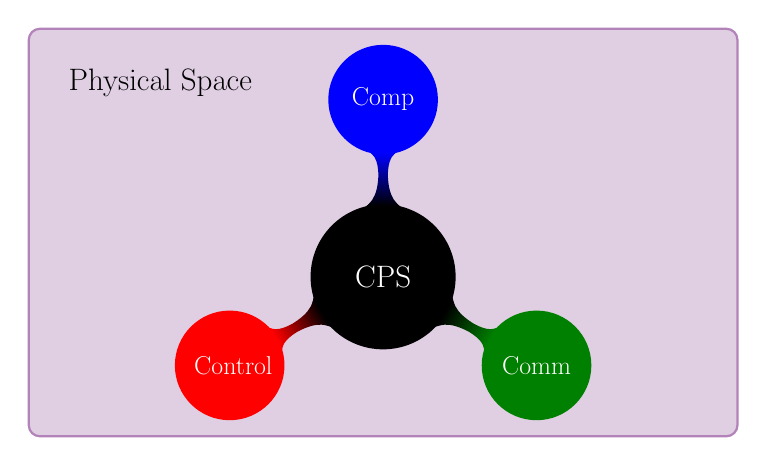
\begin{tikzpicture}[scale=0.45,transform shape,level distance=0cm,
        level 1 concept/.append style={sibling angle=120,minimum size = 3cm},
        ]
        \path [draw=thupurple!50,fill=thupurple!20,thick,rounded corners] (-10,-4.5) rectangle (10,7);
        \node at (-9,6) [anchor=north west] {\Huge Physical Space};
        \path[mindmap,concept color=black,text=white]
        node[concept] {\Huge CPS}
        [clockwise from=330]
        child[concept color=green!50!black] { node[concept](communication) {\huge Comm} }
        child[concept color=red] { node[concept](control) {\huge Control} }
        child[concept color=blue] { node[concept](computation) {\huge Comp} };
      \end{tikzpicture}
    \end{center}
  \item Applications: aerospace, chemical processes, civil infrastructure, energy, manufacturing and transportation. 
  \end{itemize}
\end{frame}

\begin{frame}{Security Threats for the CPS}
  \begin{itemize}
  \item The next generation CPS: Smart Grids, Smart Buildings, Smart Home, Internet of Things, will make extensive use of widespread sensing and networking.
  \item As the CPSs become ``smarter'', they are also more vulnerable to malicious attacks.
  \end{itemize}
  \begin{figure}[ht]
    \centering
    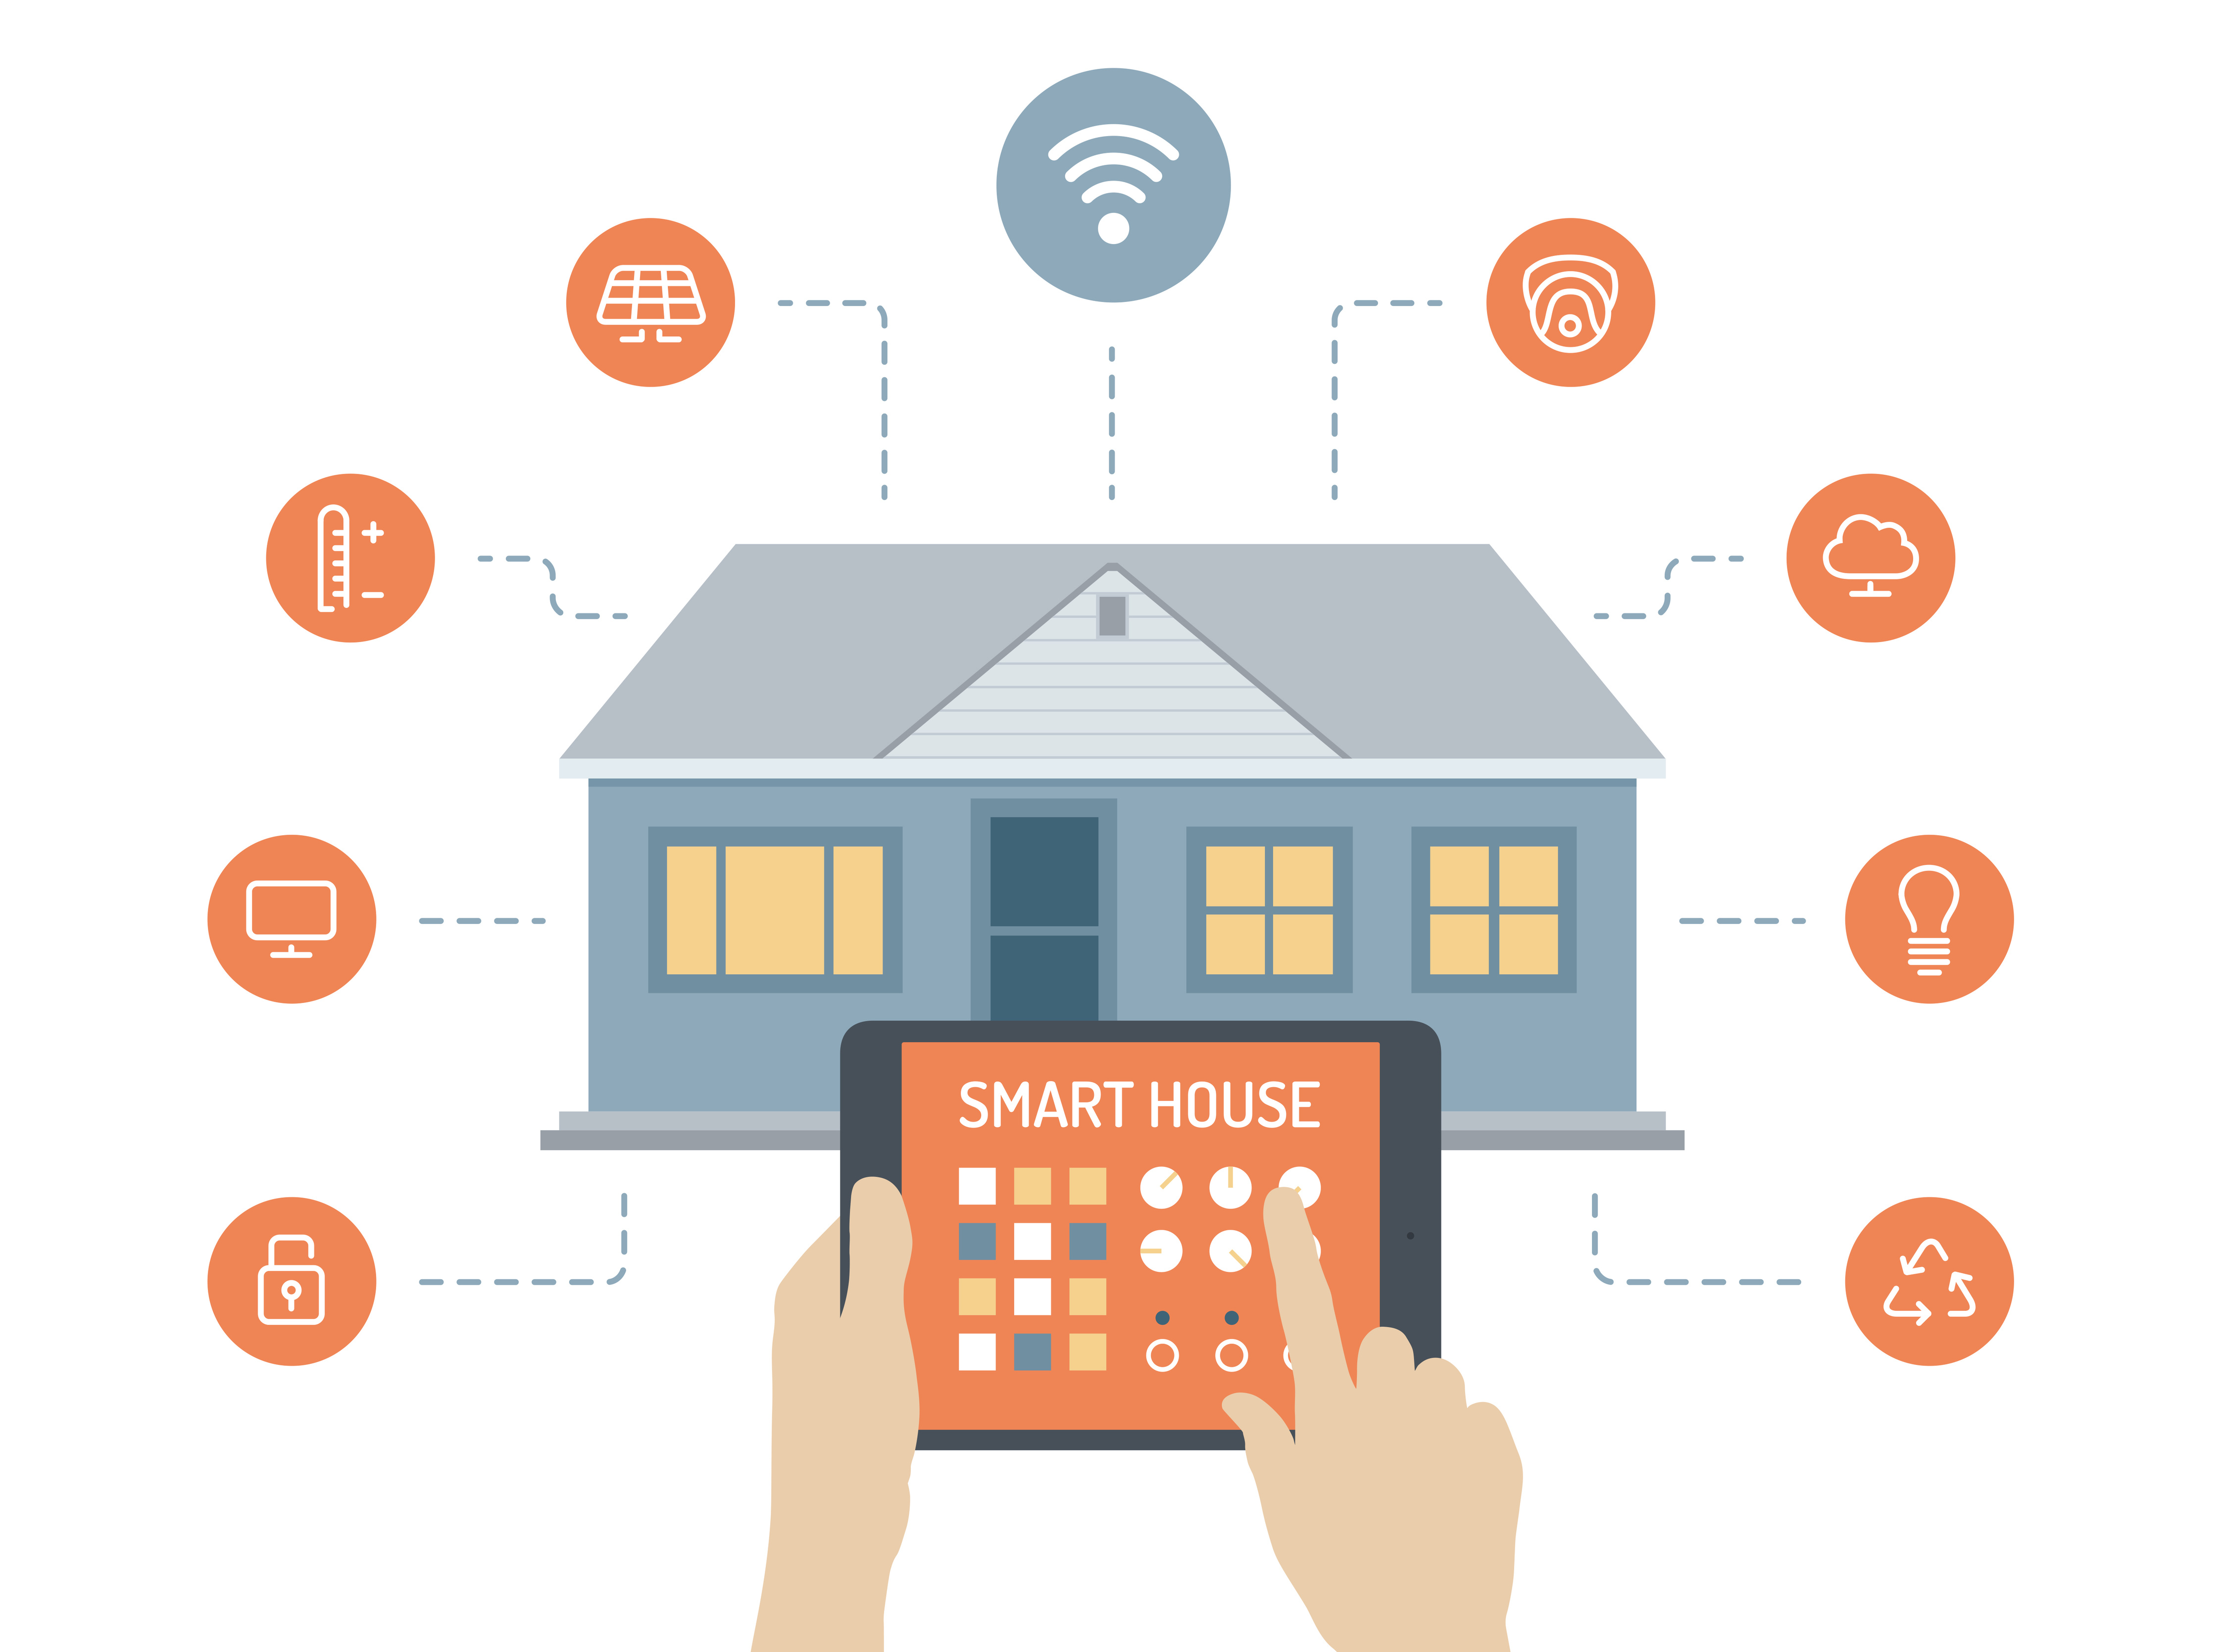
\includegraphics[width=0.6\textwidth]{SmartHome.jpg}
  \end{figure}
\end{frame}

\begin{frame}{Stuxnet}
  \begin{figure}[ht]
    \centering
    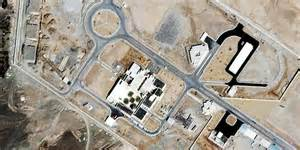
\includegraphics[width=0.8\textwidth]{stuxnet.jpg}
  \end{figure}
  Stuxnet is the first discovered malware that spies on and subverts industrial control systems. It was discovered in June 2010. 
\end{frame}

\begin{frame}{Industrial Control Systems}
  \begin{figure}[ht]
    \centering
    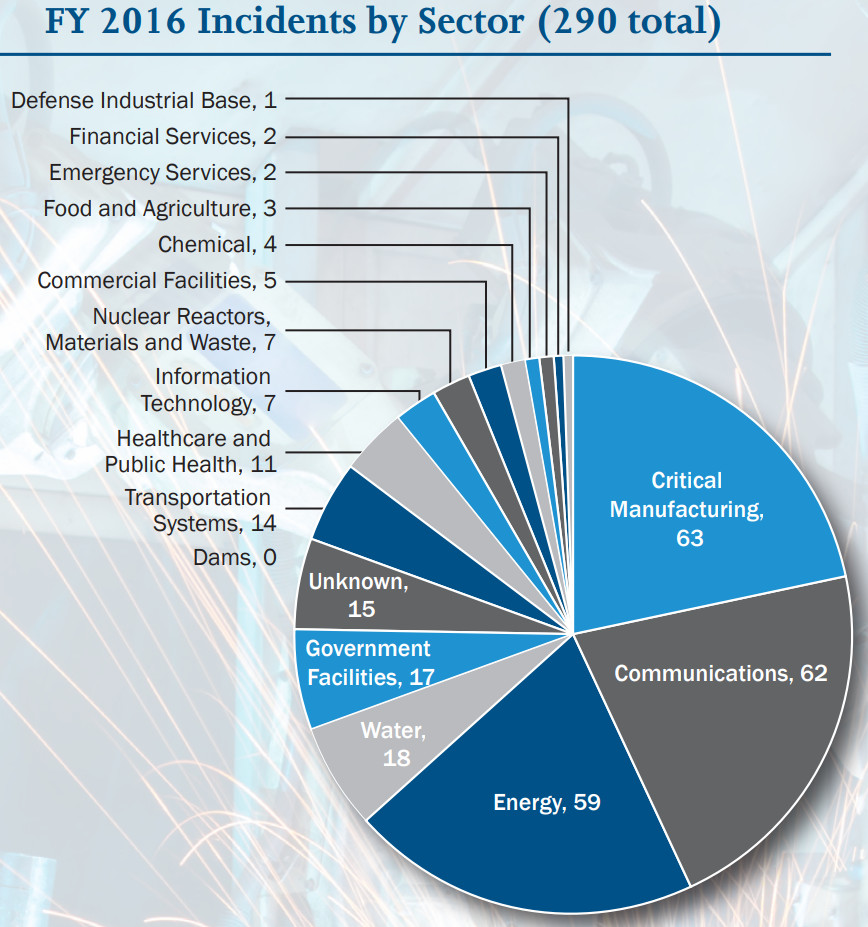
\includegraphics[width=0.6\textwidth]{cert.jpg}
  \end{figure}
 In FY 2014, ICS-CERT (Industrial Control Systems Cyber Emergency Response Team) received and responded to 245 incidents as reported by asset owners and industry partners.
\end{frame}


\begin{frame}{Industrial Control Systems}
   The scope of incidents encompassed a vast range of threats and observed methods for attempting to gain access to both business and control systems infrastructure, including but not limited to the following:
  \begin{enumerate}
  \item  Unauthorized access and exploitation of Internet facing ICS/Supervisory Control and Data Acquisition (SCADA) devices,
  \item 	 Exploitation of zero-day vulnerabilities in control system devices and software, 
  \item  	 Malware infections within air-gapped control system networks,
  \item \dots
  \end{enumerate}

\end{frame}

\begin{frame}{Attack Through Compromised Supply Chain}
  \begin{figure}[ht]
    \centering
    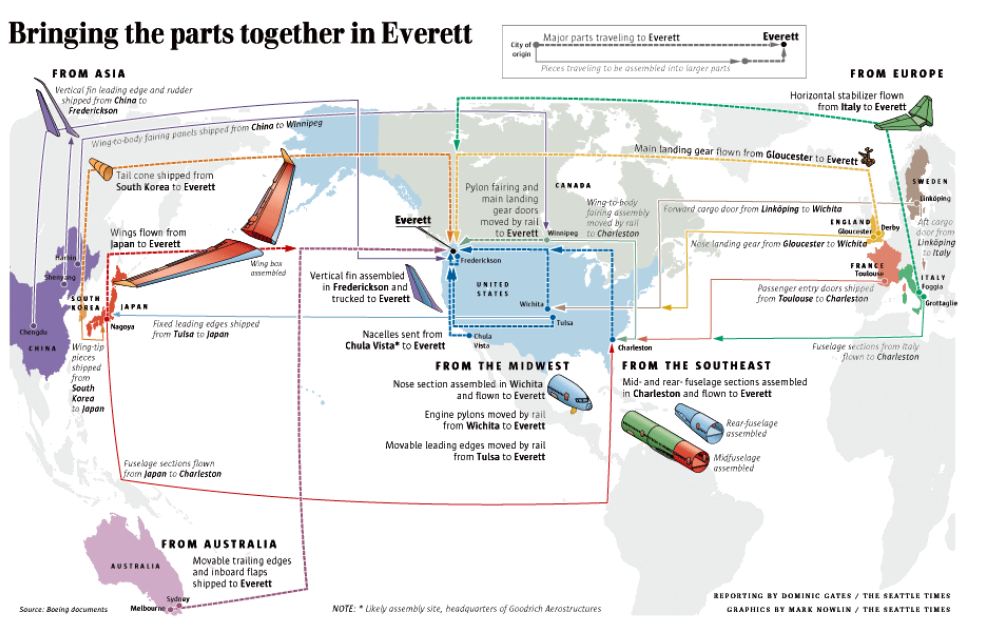
\includegraphics[width=0.8\textwidth]{boeing.jpg}
    \caption{Boeing 787 outsourced 70\% of its parts.}
  \end{figure}
\end{frame}

\begin{frame}{2003 Northeast Blackout}
  \begin{figure}[<+htpb+>]
    \begin{center}
      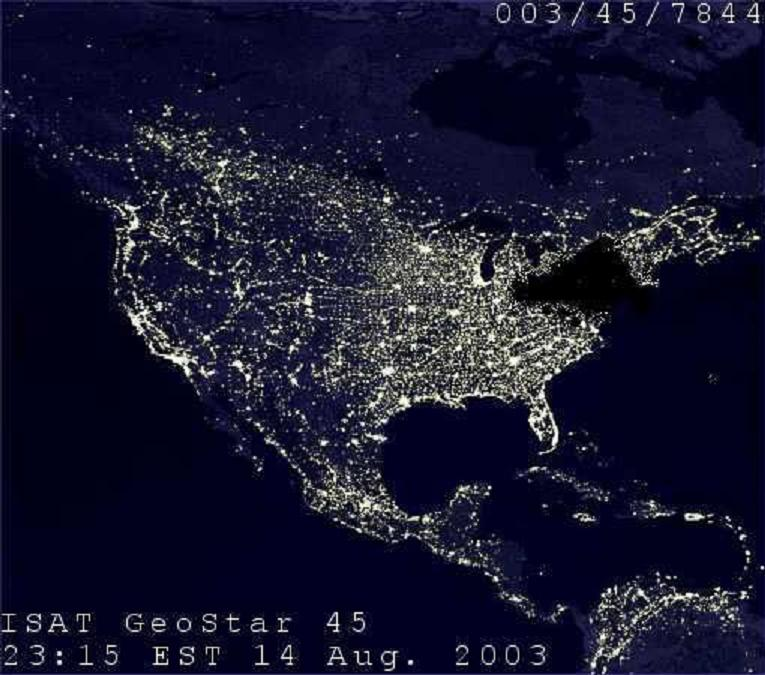
\includegraphics[width=0.60\textwidth]{blackout.jpg}
      \caption{A successful attack on CPS can have devastating effects.}
    \end{center}
  \end{figure}
\end{frame}

\begin{frame}{How to deal with CPS security threats}
  \begin{exampleblock}{}
    {\it `` If you know the enemy and know yourself, you need not fear the result of a hundred battles. If you know yourself but not the enemy, for every victory gained you will also suffer a defeat. If you know neither the enemy nor yourself, you will succumb in every battle.''}
    \vskip5mm
    \hspace*\fill{ \small--- The Art of War }
  \end{exampleblock}

  \begin{enumerate}
  \item Intrusion detection and isolation
  \item Information Fusion 
  \end{enumerate}
\end{frame}

%\begin{frame}{Overview of My Research in CPS}
%\begin{block}{Networked Control System}
%  Understanding the interaction between control and communication.
% \begin{itemize}
%  \item Kalman filtering with intermittent observation
%  \item Sensor/Actuator Scheduling: offline-schedules and event-based schedules.
%  \item Energy efficiency of consensus algorithm
% \end{itemize}
%\end{block}
%\begin{block}{CPS Security}
%\begin{itemize}
%  \item Replay attack: we proposed countermeasures to Stuxnet one year before its discovery
%  \item Deception attack
%  \item CPS security and electricity market
%  \item Information fusion
%\end{itemize}
%\end{block}

  
%\end{frame}


\begin{frame}{Hardening CPS Security using Control Theory}
  \begin{itemize}
  \item System Modelling
  \item Attack Modelling
  \item Intrusion Detection and Isolation
  \item Resilient Algorithm Design
  %\only<2>{{\color{red} Resilient Algorithm Design  }}
  \item Fundamental Limitations
  %\only <2>{{\color{red}Fundamental Limitations}}
  \item Security Investment
  %\only <2>{{\color{red}Security Investment}}
  \item \dots
  \end{itemize}
\end{frame}




%\begin{frame}{Cyber Attacks Classification}
%\large Typical attacks: \\
%  \begin{enumerate}
%  \item \large Confidentiality attack
%   \begin{itemize}
%   \item Information is disclosed to unauthorized ones (passive).
%   \end{itemize}
%  \item{\large \textcolor{red}{Integrity attack}}
%   \begin{itemize}
%   \item Modifying the data packets to compromise the data integrity (active).
%   \item Usually requiring comprehensive information about the system.
%   \end{itemize}
%  \item \large Availability attack
%   \begin{itemize}
%   \item Blocking the information change between parts of the CPS (active).
%   \item No requirement for system knowledge.
%   \end{itemize}
%  \end{enumerate}
%\end{frame}
 \section{Hypothesis Testing}
 
 \frame{\tableofcontents[currentsection]}
 \begin{frame}{A Classical Hypothesis Testing Problem}
   \begin{itemize}
   \item We want to decide whether the state $\theta$ is $-1$ or $1$.
     \begin{align*}
       \theta=\begin{cases}
         -1 &\text{w.p.~}0.5\\
         +1 &\text{w.p.~}0.5\\
       \end{cases}
     \end{align*}
   \item $m$ sensors are measuring the state: $z_i(k)\sim\mathcal N(\theta,1)$.
   \item Let us define 
     \begin{displaymath}
       z(k) = \begin{bmatrix}z_1(k)&\dots&z_m(k)\end{bmatrix},\,Z(k) = \begin{bmatrix}z(1)&\dots&z(k)\end{bmatrix}.
     \end{displaymath}
   \item A detector at time $k$  is a function $f_k:\mathbb R^{mk}\rightarrow \{-1,1\}$.
   \item A detection strategy is an infinite sequence of detectors $f = (f_1,\,f_2,\,\dots)$.
   \end{itemize}
 \end{frame}
 
 \begin{frame}{A Classical Hypothesis Testing Problem}
   \begin{center}
     \setlength{\figureheight}{2cm}
     \setlength{\figurewidth}{10cm}
     \inputtikz{gaussian}
   \end{center}
   
   Without the attacker, it is well-known that the optimal detector with minimum detection error is a Naive Bayes Detector:
   \begin{align*}
     \hat \theta(k)=f_k(Z(k))=\begin{cases}
       -1 &\text{if }\sum_{i=1}^m\sum_{t=1}^k z_i(t)/mk < 0\\
       +1 &\text{if }\sum_{i=1}^m\sum_{t=1}^k z_i(t)/mk \geq 0\\
     \end{cases}.
   \end{align*}
   
   However, the Naive Bayes Detector is not secure. Suppose the attacker compromise one sensor. Thus, it can manipulate the summation arbitrarily. Hence, it has full control over $\hat \theta$. 
 \end{frame}
 
 
 \begin{frame}{Attack Model}
   The attacker compromised $p$ sensors, the set of which is denoted as $\mathcal I$. The detector knows $p$, but does not know $\mathcal I$.
   \begin{displaymath}
     y(k) = z(k) + a(k),  
   \end{displaymath}
   where $a_i(k) = 0$ if $i\notin \mathcal I$.
   
   We consider different information set $\mathcal G(k)$ of the attacker at time $k$:
   \begin{itemize}
   \item Weak Attack Model: The attacker knows only the measurements of the compromised sensors, i.e., $\mathcal G(k) = Z_{\mathcal I}(k)$.
   \item Strong Attack Model: The attacker knows the measurements of all sensors, i.e., $\mathcal G(k) = Z(k)$. 
   \end{itemize}
   The disturbance $a(k)$ depends on the information set $\mathcal Z(k)$ and $\mathcal I$: 
   \begin{displaymath}
     a(k) = g_k(\mathcal G(k),\mathcal I). 
   \end{displaymath}
   The attack strategy $g = (g_1,\,g_2,\,\dots)$.
 \end{frame}
 
 \begin{frame}{Performance: Probability of Error}
   \begin{itemize}
   \item The probability of error at time $k$ is denoted as
     \begin{displaymath}
       P_e(k) = \max_{\mathcal I}\; P(f_k(Y(k)) \neq \theta). 
     \end{displaymath}
   \item Clearly, $P_e(k)$ is a function of the detection strategy $f$ and the attack strategy $g$.
   \item  In general, for a fixed $k$, optimizing $P_e(k)$ directly (either from the system's perspective or the attacker's perspective) is difficult.
   \item As a result, we will focus on the asymptotic performance when $k\rightarrow\infty$.
   \end{itemize}
 \end{frame}
 
 \begin{frame}{Chernoff Information}
   \begin{itemize}
   \item Suppose $m = 1$ and $p = 0$, the Naive Bayes Detector takes the following form:
     \begin{align*}
       \hat \theta(k)=f_k(Z(k))=\begin{cases}
         -1 &\text{if }\sum_{t=1}^k z_1(t)/k < 0\\
         +1 &\text{if }\sum_{t=1}^k z_1(t)/k \geq 0\\
       \end{cases}.
     \end{align*}
   \item By LLN, the probability of error goes to $0$.
   \item Moreover, it goes to $0$ exponentially fast, i.e.,
     \begin{displaymath}
       \lim_{k\rightarrow\infty}-\frac{\log P_e(k)}{k} = \max_{0<\alpha<1} -\log \int_{-\infty}^\infty \left(\frac{p^-(x)}{p^+(x)}\right)^\alpha p^+(x) dx = \frac{1}{2}.
     \end{displaymath}
   \item For general $m$ with $p = 0$, the probability of error for the Naive Bayes Detector satisfies:
     \begin{displaymath}
       P_e(k)\sim e^{-\frac{1}{2}mk}.
     \end{displaymath}
   \end{itemize}
 \end{frame}
 
 \begin{frame}{Asymptotic Performance}
   \begin{itemize}
   \item In adversarial environment, let us define the rate function $I$ as
     \begin{displaymath}
       I = \liminf_{k\rightarrow\infty} -\frac{\log P_e(k)}{k}.
     \end{displaymath}
     Roughly speaking, 
     \begin{displaymath}
       P_e(k)\sim e^{-Ik}. 
     \end{displaymath}
     Larger rate implies better detection performance.
   \item  $I$ is a function of both detection strategy $f$ and attack strategy $g$.
   \item The detector wants to maximize $I$ while the attacker wants to minimize $I$.
   \item Our goal is to find a Nash-equilibrium $(f^*,g^*)$, such that
     \begin{displaymath}
       I(f^*,g)\geq I(f^*,g^*) \geq I(f,g^*).	
     \end{displaymath}
   \end{itemize}
 \end{frame}
 
 \begin{frame}{Nash-equilibrium when $m \leq 2p$}
   \it Theorem: For both weak and strong attack model, the following strategy pair $(f^*,g^*)$ is a Nash-equilibrium with $I(f^*,g^*) = 0$:
   \begin{block}{Attack Strategy $g^*$}
     \begin{enumerate}
     \item Flip $m-p$ compromised sensors' measurements.
     \item Set the rest $2p-m$ compromised sensors' measurements to $0$. 
     \end{enumerate}
     For example, if $m=3$ and $p=2$, then the adversary should flip $1$ sensor and set the other sensor's readings to $0$.
   \end{block}
   \begin{block}{Detection Strategy $f^*$}
     $f_k = 1$ for all $k$.
   \end{block}
 \end{frame}
 \begin{frame}{Nash-Equilibrium when $m \geq 2p+1$}
   We need to define the following ``summation'' functions:
   \begin{definition}
     Define the symmetric functions $\Smin_{2p},\,\Smid_{2p},\,\Smax_{2p}:\mathbb R^{m}\rightarrow \mathbb R$ as  
     \begin{align*}
       \Smin_{2p}(x_1,\ldots,x_m) &\triangleq \sum_{i=1}^{m-2p}x_i,\\
       \Smid_{2p}(x_1,\ldots,x_m) &\triangleq \sum_{i=p+1}^{m-p}x_i,\\
       \Smax_{2p}(x_1,\ldots,x_m) &\triangleq \sum_{i=2p+1}^{m}x_i,
     \end{align*}
     when $x_1\leq \dots\leq x_m$.
   \end{definition}
 \end{frame}
 
 \begin{frame}{Nash-Equilibrium when $m \geq 2p+1$}
   \begin{itemize}
   \item If $\|x' - x\|_0\leq p$, then
     \begin{displaymath}
       \Smin_{2p}(x) \leq \Smid_{2p}(x')\leq \Smax_{2p}(x).
     \end{displaymath} 
   \item Assuming $m=5$, $p = 1$:
     \begin{center}
       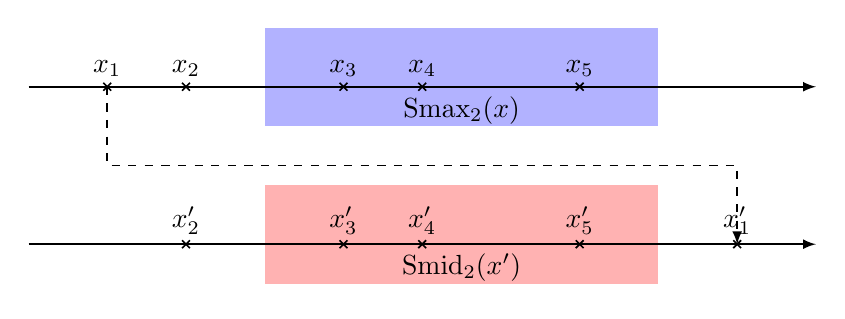
\begin{tikzpicture}[semithick,>=latex]
         \draw [->] (0,0)--(10,0);
         \draw plot[mark=x] coordinates{(1,0)} node [above] {$x_1$};
         \draw plot[mark=x] coordinates{(2,0)} node [above] {$x_2$};
         \draw plot[mark=x] coordinates{(4,0)} node [above] {$x_3$};
         \draw plot[mark=x] coordinates{(5,0)} node [above] {$x_4$};
         \draw plot[mark=x] coordinates{(7,0)} node [above] {$x_5$};
         
         \draw [->] (0,-2)--(10,-2);
         \draw plot[mark=x] coordinates{(9,-2)} node [above] {$x_1'$};
         \draw plot[mark=x] coordinates{(2,-2)} node [above] {$x_2'$};
         \draw plot[mark=x] coordinates{(4,-2)} node [above] {$x_3'$};
         \draw plot[mark=x] coordinates{(5,-2)} node [above] {$x_4'$};
         \draw plot[mark=x] coordinates{(7,-2)} node [above] {$x_5'$};
         
         \draw [->,dashed] (1,0)--(1,-1)--(9,-1)--(9,-2);
         \begin{pgfonlayer}{background}
           \fill [fill=red!30] (3,-2.5) rectangle (8,-1.25);
           \node at (5.5,-2.3) {$\Smid_2(x')$};
           
           \fill [fill=blue!30] (3,-0.5) rectangle (8,0.75);
           \node at (5.5,-0.3) {$\Smax_2(x)$};
         \end{pgfonlayer}
       \end{tikzpicture}
     \end{center}
   \item $\Smid_{2p}$ is a more ``secure'' version of sum. 
   \end{itemize}
 \end{frame}
 
 
 \begin{frame}{Nash-Equilibrium when $m \geq 2p+1$}
   \it Theorem: For both weak and strong attack model, the following strategy pair $(f^*,g^*)$ is a Nash-equilibrium with $I(f^*,g^*) = (m-2p)/2$:
   \begin{block}{Attack Strategy $g^*$}
     Flip $p$ compromised sensors' measurements.
   \end{block}
   \begin{block}{Detection Strategy $f^*$}
     \begin{enumerate}
     \item For each sensor $i$, compute a local sum $ \Lambda_i(k) = \sum_{t=1}^k y_i(t)$.
     \item The detector $f_k$ is given by
       \begin{displaymath}
         f_k(Y(k)) = \begin{cases}
           -1 &\text{if }\Smid_{2p}(\Lambda(k))< 0\\
           1 &\text{if }\Smid_{2p}(\Lambda(k))\geq 0\\
         \end{cases}
       \end{displaymath}
     \item At each time step, the computation is $O(m)$.
     \end{enumerate}
   \end{block}
 \end{frame}
 
 \begin{frame}{Numerical Examples}
   We assume $m = 9$ and plot the probability of error for the equilibrium strategy for different $p$
   \begin{center}
     \setlength{\figureheight}{7cm}
     \setlength{\figurewidth}{12cm}
     \inputtikz{Perror}
   \end{center}
 \end{frame}
 
 \begin{frame}{What if the defender does not know $p$?}
   \begin{enumerate}
   \item Suppose the defender does not know $p$, and implement a detector assuming using $\Smid_{2p'}$.
   \item If $p' \geq p$, then the detector is still resilient to the attack, with rate $(m-p-p')/2$ (comparing to the optimal rate $(m-2p)/2$)
   \item If $p' < p$, then the detector is not resilient. The rate will be $0$.
   \end{enumerate}
   
   \centering
   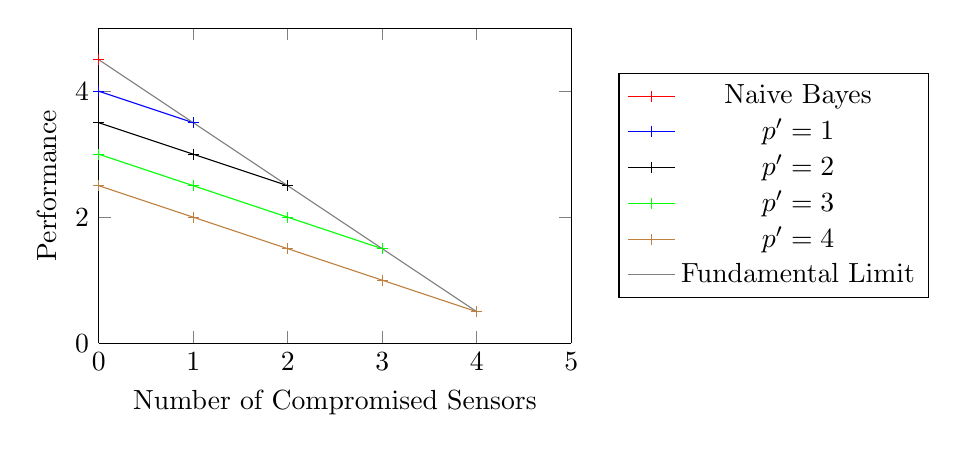
\begin{tikzpicture}
     \begin{axis}[%
       width=6cm,
       height=4cm,
       scale only axis,
       separate axis lines,
       every outer x axis line/.append style={black},
       every x tick label/.append style={font=\color{black}},
       xmin=0,
       xmax=5,
       xlabel={Number of Compromised Sensors},
       every outer y axis line/.append style={black},
       every y tick label/.append style={font=\color{black}},
       ymin=0,
       ymax=5,
       ylabel={Performance},
       axis background/.style={fill=white},
       legend style={at={(1.1,0.5)},anchor=west},
       ]
       \addplot [color=red,solid,mark=+]
       table[row sep=crcr]{%
       0	4.5\\
     };
       \addlegendentry{Naive Bayes};
       
       \addplot [color=blue,solid,mark=+]
       table[row sep=crcr]{%
       0	4\\
       1	3.5\\
     };
       \addlegendentry{$p' = 1$};
       
       \addplot [color=black,solid,mark=+]
       table[row sep=crcr]{%
       0	3.5\\
       1	3\\
       2	2.5\\
     };
       \addlegendentry{$p' = 2$};
       
       \addplot [color=green,solid,mark=+]
       table[row sep=crcr]{%
       0	3\\
       1	2.5\\
       2	2\\
       3	1.5\\
     };
       \addlegendentry{$p' = 3$};
       
       
       \addplot [color=brown,solid,mark=+]
       table[row sep=crcr]{%
       0	2.5\\
       1	2\\
       2	1.5\\
       3	1\\
       4	0.5\\
     };
       \addlegendentry{$p' = 4$};
       
       \addplot [color=gray,solid]
       table[row sep=crcr]{%
       0	4.5\\
       1	3.5\\
       2	2.5\\
       3	1.5\\
       4	0.5\\
     };
       \addlegendentry{Fundamental Limit};
     \end{axis}
   \end{tikzpicture}
   
 \end{frame}


\section{Trade-off Between Efficiency and Security}
\begin{frame}{Outline}
  \tableofcontents[currentsection]
\end{frame}
%\begin{frame}{Binary Hypothesis Testing}
%   We want to detect certain event:
%    \begin{align*}
%      \theta=\begin{cases}
%        0 &\text{w.p.~}0.5\\
%        1 &\text{w.p.~}0.5\\
%      \end{cases},
%    \end{align*}
%    with $m$ homogeneous  sensors measuring the system.
%\end{frame}
%
%
%
%\begin{frame}{Attack Modelling}
%\begin{itemize}
%  \item The adversary can change up to $n$ sensors' measurements arbitrarily, which can be achieved by
%  \begin{enumerate}
%  \item Compromising the sensors' hardware/software
%  \item Hijacking the communication from sensors
%  \item Physical attacks
%  \end{enumerate}
%  \vspace{2mm}
%  \item The system knows $n$, but does not know what sensors are compromised.
%\end{itemize}
%\end{frame}
%
%\begin{frame}{Motivating Example}
%  \begin{center}
%    \setlength{\figureheight}{2cm}
%    \setlength{\figurewidth}{10cm}
%    \inputtikz{gaussian}
%  \end{center}
%  \begin{block}{Naive Probability Ratio Test: Optimal Without Attacks}
%  \begin{enumerate}
%  \item  Compute the average of all measurements and compare it with 0.
%  \item  Choose $\hat \theta = 0$ if the average is less than 0.
%  Choose $\hat \theta = 1$ otherwise.
%  \end{enumerate}
%  \end{block}
%%  \begin{itemize}
%%  \item The optimal fusion algorithm is to
%%  \item Choose $\hat \theta = 0$ if the average is less than 0.
%%  \item Choose $\hat \theta = 1$ otherwise.
%%  \item However, this is not secure.
%%  \end{itemize}
%\begin{center}
% \only <2> {\large{ {\color{red}not secure at all}}}
%\end{center}
%\end{frame}
%
%
%
%\begin{frame}{Cost of Security}
%  \begin{itemize}
%  \item Security: The performance of the information fusion algorithm when under attack
%        \begin{align*}
%    \liminf_{k\rightarrow\infty} - \frac{\log \max_g\{\pr(f_k=1|0),\pr(f_k=0|1)\}}{k}
%  \end{align*}
% % \item However, there may be a cost associated with security, as we cannot use the optimal (but non-secure) fusion algorithm.
%  \item Efficiency: The performance of the fusion algorithm when all sensors are benign.
%          \begin{align*}
%    \liminf_{k\rightarrow\infty} - \frac{\log \max\{\pr(f_k=1|0),\pr(f_k=0|1)\}}{k}
%  \end{align*}
%  \item What is best achievable trade-off between security and efficiency?
%  \end{itemize}
%\end{frame}
%
%
%
%
%
%
%\begin{frame}{General Case}
%      \begin{center}
%        \inputtikz{fun_lim}
%      \end{center}
%\vspace{-5mm}
%$C$: biggest contribution that one healthy sensor can provide
%         \begin{align*}
%    C\triangleq \liminf_{k\rightarrow\infty} - \frac{\log \max\{\pr(f^*_k=1|0),\pr(f^*_k=0|1)\}}{k}
%  \end{align*}
%  where $f^*$ is the classic probability ratio test.
%\end{frame}

\begin{frame}{Binary Hypothesis Testing Under Attack}
  \begin{center}
    \setlength{\figureheight}{2cm}
    \setlength{\figurewidth}{10cm}
    \inputtikz{blockdiagram}
  \end{center}
\begin{itemize}
  \item Up to $n$ sensors' measurements arbitrarily manipulated
  \begin{enumerate}
  \item Compromising the sensors' hardware/software
  \item Hijacking the communication from sensors
  \item Physical attacks
  \end{enumerate}
  \vspace{2mm}
  \item The system knows $n$, but does not know what sensors are compromised.
\end{itemize}
\end{frame}


\begin{frame}{Motivating Example: Classic Probability Ratio Test}
    \begin{center}
    \setlength{\figureheight}{2cm}
    \setlength{\figurewidth}{10cm}
    \inputtikz{blockdiagram}
  \end{center}
\begin{itemize}
  \item At each time $k$, classic probability ratio test runs as
  \begin{align*}
        \theta = \begin{cases}
        0 & \text{if } \sum_{t=1}^{k}\sum_{i=1}^m L(\tilde y_i(t)) \leq 0\\
        1 & \text{if } \sum_{t=1}^{k}\sum_{i=1}^m L(\tilde y_i(t)) > 0,
        \end{cases}
  \end{align*}
  where $L(\tilde y_i(k))$ is the log-likelihood ratio.
  \item Optimal without attacks
\end{itemize}
\begin{center}
 \only <2> {\Large{ {\color{red}not secure at all}}}
\end{center}
\end{frame}

\begin{frame}{Motivating Example: Trimmed Mean Algorithm}
    \begin{center}
    \setlength{\figureheight}{2cm}
    \setlength{\figurewidth}{10cm}
    \inputtikz{blockdiagram}
  \end{center}
\begin{itemize}
  \item At each time $k$, trimmed mean algorithm runs as
   \begin{enumerate}
     \item Remove the measurements with the largest $n$ and smallest $n$ log-likelihood ratios;
     \item Apply classic probability ratio test to the remaining $m-2n$ data
   \end{enumerate}
\end{itemize}
\begin{center}
 \only <2> {\Large{ {\color{red}too conservative?}}}
\end{center}
\end{frame}







\begin{frame}{Tradeoff Between Security and Efficiency}
  \begin{itemize}
  \item Security: The performance of the information fusion algorithm when under attack
        \begin{align*}
    \liminf_{k\rightarrow\infty} - \frac{\log \max_{g,\theta} \pr(f_k\neq \theta|\theta)}{k}
  \end{align*}
 % \item However, there may be a cost associated with security, as we cannot use the optimal (but non-secure) fusion algorithm.
  \item Efficiency: The performance of the fusion algorithm when all sensors are benign.
          \begin{align*}
    \liminf_{k\rightarrow\infty} - \frac{\log \max_{\theta} \pr(f_k\neq \theta|\theta)}{k}
  \end{align*}
  \item What is best achievable trade-off between security and efficiency?
  \end{itemize}
\end{frame}

\begin{frame}{Main Results}
      \begin{center}
        \inputtikz{fun_lim}
      \end{center}
\vspace{-5mm}
$C$: biggest contribution that one healthy sensor can provide
         \begin{align*}
    C\triangleq    \liminf_{k\rightarrow\infty} - \frac{\log \max_{\theta} \pr(f_k^*\neq \theta|\theta)}{k}
  \end{align*}
  where $f^*$ is the classic probability ratio test.
\end{frame}






\begin{frame}{Proofs of Upper Bounds}
\begin{itemize}
\item The best achievable efficiency is $mC$.
\begin{itemize}
\item
Classic probability ratio test
\end{itemize}
\visible<2->{\item  The best achievable security is $(m-2n)C$.
\begin{itemize}
\item
The achievability is deferred
\item The limit is shown by construct the following attack strategy.
  \begin{center}
    \setlength{\figureheight}{2cm}
    \setlength{\figurewidth}{10cm}
    \inputtikz{attack}
  \end{center}
green/red: healthy/compromised sensors\\
circle/triangle: different distributions}
\end{itemize}

\end{itemize}
\end{frame}



\begin{frame}{Fundamental Limits of Trade-off}
\begin{itemize}
\item Consider the following two hypotheses:
  \begin{center}
    \setlength{\figureheight}{2cm}
    \setlength{\figurewidth}{10cm}
    \inputtikz{lim1}
  \end{center}
Suppose that we aim to find a detector such that the following is minimized.
\[\pr(f=1|0) + \phi\pr(f=0|1). \]

\item Bayesian detection theory $\Longrightarrow$ fundamental relation between $\pr(f=1|0)$ and $\pr(f=0|1)$.

\visible<2->{\item Efficiency $\leq \pr(f=1|0)$, Security $\leq \pr(f=0|1)$}
\visible<3->{\item Vary $\phi$}
\end{itemize}
\end{frame}



\begin{frame}{Fundamental Limits of Trade-off: Cont'd}
\begin{itemize}
\item Consider the following two hypotheses:
  \begin{center}
    \setlength{\figureheight}{2cm}
    \setlength{\figurewidth}{10cm}
    \inputtikz{lim2}
  \end{center}
\end{itemize}
\end{frame}

\begin{frame}{Achievability}
 There exists algorithms achieving the limits, i.e., the limit is tight.
   \begin{enumerate}
   \item Each of the $m$ measurements is mapped to \emph{nonnegative} numbers by two functions $I_0,I_1$.
  \item If there are $m-n$ values of $I_0$ whose sum is ``small'' enough, then choose $\hat \theta = 0$.
  \item If there are $m-n$ values of $I_1$ whose sum is ``small'' enough, then choose $\hat \theta = 1$.
  \item Compare the average of log-likelihood ratios with 0 to decide if $\hat \theta = 0$ or $1$.
  \end{enumerate}
\end{frame}


\begin{frame}{Intuitions of the Algorithm}
 \begin{itemize}
   \item  Nonnegative mapping.
     \begin{center}
    \setlength{\figureheight}{2cm}
    \setlength{\figurewidth}{10cm}
    \inputtikz{nonnegative}
  \end{center}
  \item Safe kernel
       \begin{center}
    \setlength{\figureheight}{2cm}
    \setlength{\figurewidth}{10cm}
    \inputtikz{safekernel}
  \end{center}
  \end{itemize}
\end{frame}






\begin{frame}{Gaussian Cases}
\begin{itemize}
\item The best security $(m-2n)C$ and the best efficiency $mC$ are achieved simultaneously
\item Security is cost-free
\begin{itemize}
  \item Computational burden: $O(m)$ versus $O(m\log m)$
\end{itemize}
\item More than Gaussian: ``symmetric" distributions. There exists a constant $a$ such that for any Borel measurable set $\mathcal A$,
\begin{align*}
  \mu(a+\mathcal A) = \nu (a-\mathcal A).
\end{align*}
\end{itemize}
\end{frame}


\begin{frame}{Non-Asymptotic Performance}
      \begin{center}
        \inputtikz{finite_time}
      \end{center}
\end{frame}



\begin{frame}{Secure Sensors}
\begin{itemize}
\item A subset of sensors are well protected and cannot be compromised.
\item Trade-offs?
\item Similar ideas to prove limits and design algorithm?
\end{itemize}
\end{frame}

\begin{frame}{Fundamental Trade-off when There are Secure Sensors}
$m_s$ normal sensors are replaced with secure ones.
\begin{itemize}
\item $2n \leq m-m_s$: nothing affected
\begin{itemize}
  \item The redundancy of the $m-m_s$ normal sensors is enough
\end{itemize}
\item $2n > m-m_s$: the trade-off limit remains, and the maximum security level is increased from $\max(0,(m-2n)C)$ to $m_sC$
\item Do nothing or secure more than $m-2n$ sensors
\end{itemize}
\end{frame}

\begin{frame}{Detection Algorithm when There are Secure Sensors}
   \begin{enumerate}
   \item Mapping by nonnegative functions $I_0,I_1$.
  \item Sum $I_0$ of the $m_s$ secure sensors and any $m-m_s-n$ of $I_0$ of the $m-m_s$ normal sensors, if there exist one ``small'' enough, then choose $\hat \theta = 0$.
  \item Sum $I_1$ of the $m_s$ secure sensors and any $m-m_s-n$ of $I_1$ of the $m-m_s$ normal sensors, if there exist one ``small'' enough, then choose $\hat \theta = 1$.
  \item Compare with $0$.
  \end{enumerate}
\end{frame}




%\begin{frame}{Unknown Number of Compromised Sensors}
%   \begin{itemize}
%     \item The number of sensors being attacked, $n_a$,  is in a set, size of which is more than $2$
%     \item $n_a\in\{0,n\}$ for security/efficiency case
%     \item Trade-offs among these ``multi-level" detection performances?
%   \end{itemize}
%\end{frame}
%
%\begin{frame}{Fundamental Trade-off and Algorithm when the Number of Compromised Sensors is Unknown}
%   \begin{itemize}
%     \item Pairwise trade-off for any two $n_a$ $\Longrightarrow$  trade-off on the whole set
%     \item Pairwise trade-off is obtained using the aforementioned idea
%   \visible<2->{  \item The algorithm achieving the ``multi-level" limits is:
%   \begin{enumerate}
%   \item Mapping by two nonnegative functions $I_0,I_1$.
%   \item For any sequence of $n_a\geq 1$ in the set,
%   \begin{itemize}
%  \item If there are $m-n_a$ values of $I_0$ whose sum is ``small'' enough, then choose $\hat \theta = 0$.
%  \item If there are $m-n_a$ values of $I_1$ whose sum is ``small'' enough, then choose $\hat \theta = 1$.
%  \end{itemize}
%  \item Compare with $0$
%  \end{enumerate}}
%   \end{itemize}
%\end{frame}


\section{Static State Estimation}

\begin{frame}{Preliminary: Static State Estimation}
  \begin{enumerate}
  \item We assume that $x \in \mathbb R^n$ is the state that we want to estimate.
  \item $m$ sensors are deployed to monitor the system. Denote $z_i \in \mathbb R$ as the measurement generated by sensor $i$.
  \item Denote $z = \begin{bmatrix}z_1&\dots&z_m\end{bmatrix}^T$ as the collection of all sensory data.
  \item We assume the following sensor model:
    \begin{align*}
      z = Hx + w,
    \end{align*}
    where $H$ is a matrix of proper dimension and $w$ represent random noise.
  \item The optimal state estimator is of the form
    \begin{align*}
      \hat x = Kz, \text{ where }K = (H^TH)^{-1}H^T.
    \end{align*}
  \end{enumerate}
\end{frame}

\begin{frame}{Preliminary: Secure State Estimation}
  Suppose the following sensory model:
  \begin{align*}
    y = \begin{bmatrix}
      1\\
      1\\
      1
    \end{bmatrix}x + w.
  \end{align*}
  The optimal estimator is given by
  \begin{align*}
    \hat x = \frac{1}{3}\left(y_1+y_2+y_3\right).
  \end{align*}
  
  This estimator is not resilient to a single malicious sensor.
\end{frame}

\begin{frame}{Problem Formulation}
  \begin{enumerate}
  \item Assume that at most $p$ sensors are compromised.
  \item The sensory model is given by
    \begin{align*}
      y = z + a = Hx + w +a,
    \end{align*}
    where $a$ is a $p$-sparse vector indicating the attacker's action.
  \item We will call an estimator $\hat x = g(y)$ to be resilient if
    \begin{align*}
      \|g(y) - g(z)\|\text{ is bounded for all $p$-sparse $a$}.
    \end{align*}
  \item The total state estimation error can be written as
    \begin{align*}
      x-g(y) = x-g(z) + g(z)-g(y).
    \end{align*}

    \emph{Resiliency means that the state estimation error caused by the adversary is bounded!}
  \end{enumerate}
\end{frame}

\begin{frame}{Why do not use information security}
  \begin{itemize}
  \item Tamper-resistant microprocessor, Software attestation, Secure Communication Protocol,\dots
  \item It is hard to guarantee security for every single sensor. (A single compromised sensor can totally ruin the linear estimator.)
  \item Physical attacks?
  \item A resilient estimator can provide an additional layer of protection.
  \end{itemize}
\end{frame}

\begin{frame}{Why not use bad data detection?}
  \begin{center}
    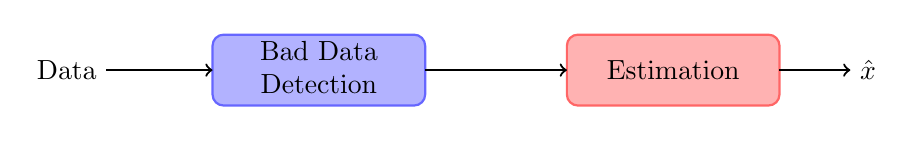
\begin{tikzpicture}[scale=0.9]
      \draw[thick,rounded corners,fill=blue!30,draw=blue!60] (0,1) rectangle (3,2);
      \node at (1.5,1.5) {\begin{tabular}{c} Bad Data\\ Detection \end{tabular}};
      \draw[thick,rounded corners,fill=red!30,draw=red!60] (5,1) rectangle (8,2);
      \node at (6.5,1.5) {Estimation};
      \draw[thick,->] (-1.5,1.5)--(0,1.5);
      \node [anchor=east] at (-1.5,1.5) {Data};
      \draw[thick,->] (3,1.5) to (5,1.5);
      \draw[thick,->] (8,1.5) to (9,1.5);
      \node [anchor=west] at (9,1.5) {$\hat x$};
    \end{tikzpicture}
  \end{center}
  \begin{enumerate}
  \item A typical bad data detector will first compute $\hat x = Ky$ and then the residue $r = y - H\hat x$.
  \item The bad data detector will then remove the sensors with large residue.
  \item Drawbacks: It is designed for \emph{random failures}, not necessarily attacks; Difficult to analyze the estimation performance.
  \end{enumerate}
\end{frame}

\begin{frame}{Why not use bad data detection?}
  \begin{center}

    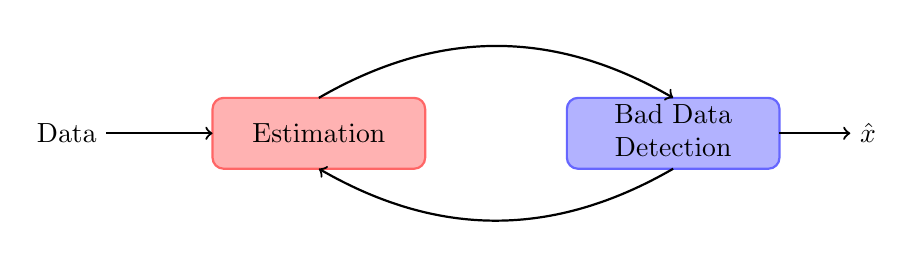
\begin{tikzpicture}[scale=0.9]
      \draw[thick,rounded corners,fill=red!30,draw=red!60] (0,1) rectangle (3,2);
      \node at (1.5,1.5) {Estimation};

      \draw[thick,rounded corners,fill=blue!30,draw=blue!60] (5,1) rectangle (8,2);
      \node at (6.5,1.5) {\begin{tabular}{c} Bad Data\\ Detection \end{tabular}};

      \draw[thick,->] (-1.5,1.5)--(0,1.5);
      \node [anchor=east] at (-1.5,1.5) {Data};

      % \draw[thick,->] (3,1.5) to (5,1.5);

      \draw[thick,->] (1.5,2) to [bend left] (6.5,2);
      \draw[thick,->] (6.5,1) to [bend left] (1.5,1);

      \draw[thick,->] (8,1.5) to (9,1.5);

      \node [anchor=west] at (9,1.5) {$\hat x$};
    \end{tikzpicture}
  \end{center}
  \begin{enumerate}
  \item A typical bad data detector will first compute $\hat x = Ky$ and then the residue $r = y - H\hat x$.
  \item The bad data detector will then remove the sensors with large residue.
  \item Drawbacks: It is designed for \emph{random failures}, not necessarily attacks; Difficult to analyze the estimation performance.
  \end{enumerate}
\end{frame}

\begin{frame}{Some Related Research}
  \begin{enumerate}
    % \item For the noiseless case, i.e., $w = 0$ we know that
    %   \begin{itemize}
    %   \item If for any $x\neq 0$, $\|Hx\|_0 \geq p+1$, then we can detect the existence of compromised sensors.
    %   \item If for any $x\neq 0$, $\|Hx\|_0 \geq 2p+1$, then we can isolate the set of compromised sensors and reconstruct $x$.
    %   \end{itemize}
  \item The following estimator is resilient:
    \begin{align*}
      & \mathop{\textit{minimize}}\limits_{\hat x,a,w}&
      & \|w\|^2 \\
      &\text{subject to}&
      &y = H \hat x + w + a,\,\|a\|_0\leq p.
    \end{align*}
    The drawback: The optimization problem is not convex and solving it is computationally difficult.
  \item We can use convex optimization based estimator, e.g., 
    \begin{align*}
      & \mathop{\textit{minimize}}\limits_{\hat x,a,w}&
      & \|w\|^2 + \|a\|_1 \\
      &\text{subject to}&
      &y = H \hat x + w + a.
    \end{align*}
    However, there is no guarantee on the resiliency.
  \end{enumerate}
\end{frame}

\begin{frame}{A General Convex Optimization Based Estimator}
  We consider the following estimator
  \begin{align*}
    \hat x = g(y) \triangleq \argmin_{\hat x} \sum_{i=1}^m f_i(y_i-H_i \hat x),
  \end{align*}
  where the following properties of function $f_i:\mathbb R\mapsto \mathbb R$ are assumed:
  \begin{enumerate}
  \item $f_i$ is convex.
  \item $f_i$ is symmetric, i.e., $f_i(u) = f_i(-u)$.
  \item $f_i$ is non-negative and $f_i(0) = 0$.
  \end{enumerate} 

  If we define the residue $r_i\triangleq y_i - H_i\hat x$, then we are trying to minimize the sum of some cost function related to the residue.

  The estimator can be computed efficiently via convex optimization. (It is also easy be computed in a parallel fashion.)
\end{frame}


\begin{frame}{A General Convex Optimization Based Estimator}
  Our proposed estimator is very general since we can choose the right $f_i$ to get the following estimator:
  \begin{enumerate}
  \item Linear Estimator:
    \begin{align*}
      g(y) = \argmin_{\hat x} \|y-H\hat x\|_2^2= \argmin_{\hat x}  \sum_{i=1}^m (y_i-H_i\hat x)^2.
    \end{align*}
  \item $L_1$ Estimator:
    \begin{align*}
      g(y) = \argmin_{\hat x} \|y-H\hat x\|_1=\argmin_{\hat x} \sum_{i=1}^m |y_i-H_i\hat x|.
    \end{align*}
  \end{enumerate}
\end{frame}


\begin{frame}{A General Convex Optimization Based Estimator}
  \begin{enumerate}  \setcounter{enumi}{2}

  \item LASSO:
    \begin{align*}
      g(y) = \argmin_{\hat x} \|w\|^2+\lambda \|a\|_1, \text{ s.t. }y=H\hat x+w+a.
    \end{align*}
    We can define $r_i = y_i-H_i\hat x = w_i+a_i$. Then the problem can be rewritten as
    \begin{align*}
      g(y) = \argmin_{\hat x}\sum_{i=1}^m \min_{w_i}\left(\|w_i\|^2+\lambda \|r_i-w_i\|_1\right), \text{ s.t. }r_i=y_i-H\hat x.
    \end{align*}
    As a result, we can rewrite $g$ as
    \begin{align*}
      g(y) = \argmin_{\hat x} \sum_{i=1}^m f(y_i-H_i\hat x)
    \end{align*}
    where $f(r) = \min_{w} w^2 + \lambda |r-w|.$
  \end{enumerate}
\end{frame}

\begin{frame}{Example}
  Suppose the following sensory model:
  \begin{align*}
    y = \begin{bmatrix}
      1\\
      1\\
      1
    \end{bmatrix}x + w+a,\,\|a\|_0\leq 1.
  \end{align*}
  Then the following estimator is resilient (in fact, it is the median of $y_i$):
  \begin{align*}
    g(y) = \argmin_{\hat x}  |y_1-\hat x|+|y_2-\hat x|+|y_3-\hat x|.
  \end{align*}
\end{frame}

\begin{frame}{Example}
  \begin{figure}[ht]
    \centering
    \begin{tikzpicture}[yscale=0.4]
      \draw[thick,->] (0,0)--(9,0);
      \node [anchor=west] at (9,0) {$\hat x$};
      \draw[thin,gray] (2,0)--(2,0.1);
      \draw[thin,gray] (5,0)--(5,0.1);
      \draw[thin,gray] (7,0)--(7,0.1);
      \draw[thick](1,11)--(2,8)--(5,5)--(7,7)--(8,10);
      \node [anchor=north] at (2,0) {\color{red}{$y_1$}};
      \node [anchor=north] at (5,0) {\color{blue}{$y_2$}};
      \node [anchor=north] at (7,0) {\color{brown}{$y_3$}};
    \end{tikzpicture}
  \end{figure}
  \color{white}{If we interpret the function $|y_i-\hat x|$ as a potential function generate by sensor $i$, then we can see that sensor $i$ is dragging $\hat x$ towards $y_i$ with $1$ unit of force. The equilibrium point will be at the middle $y_i$.}
\end{frame}

\begin{frame}{Interpretation}
  \begin{figure}[ht]
    \centering
    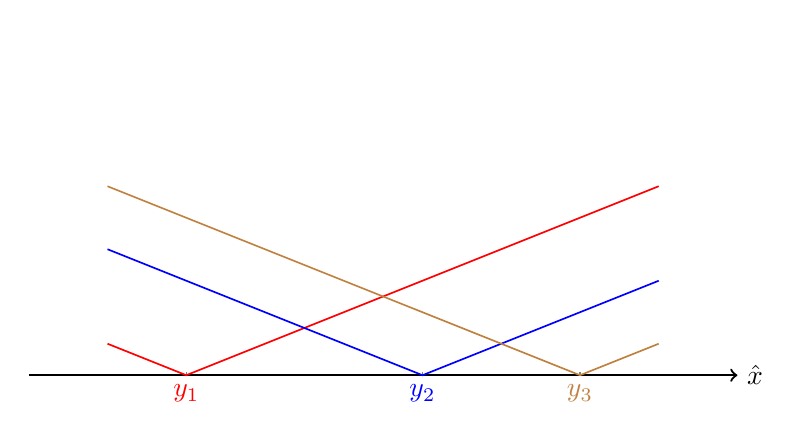
\begin{tikzpicture}[yscale=0.4]
      \draw[thick,->] (0,0)--(9,0);
      \node [anchor=west] at (9,0) {$\hat x$};
      \draw[thin,gray] (2,0)--(2,0.1);
      \draw[thin,gray] (5,0)--(5,0.1);
      \draw[thin,gray] (7,0)--(7,0.1);
      \draw[thick,white](1,11)--(2,8)--(5,5)--(7,7)--(8,10);
      \node [anchor=north] at (2,0) {\color{red}{$y_1$}};
      \draw[semithick,red](1,1)--(2,0)--(8,6);
      \node [anchor=north] at (5,0) {\color{blue}{$y_2$}};
      \draw[semithick,blue](1,4)--(5,0)--(8,3);
      \node [anchor=north] at (7,0) {\color{brown}{$y_3$}};
      \draw[semithick,brown](1,6)--(7,0)--(8,1);
    \end{tikzpicture}
  \end{figure}
  If we interpret the function $|y_i-\hat x|$ as a potential function generate by sensor $i$, then we can see that sensor $i$ is dragging $\hat x$ towards $y_i$ with $1$ unit of force. The equilibrium point will be at the middle $y_i$.
\end{frame}

\begin{frame}{Another Example}
  Suppose the following sensory model:
  \begin{align*}
    y = \begin{bmatrix}
      1\\
      1\\
      3
    \end{bmatrix}x + w+a ,\,\|a\|_0\leq 1.
  \end{align*}
  Then the following estimator is not resilient:
  \begin{align*}
    g(y) = \argmin_{\hat x}  |y_1-\hat x|+|y_2-\hat x|+|y_3-3\hat x|.
  \end{align*}
  In fact, we can rewrite it as
  \begin{align*}
    g(y) = \argmin_{\hat x}  |y_1-\hat x|+|y_2-\hat x|+3\left|\frac{y_3}{3}-\hat x\right| = \frac{y_3}{3}
  \end{align*}
  Sensor $3$ generates $3$ unit of force comparing to $1$ unit of force from sensor $1$ and $2$.
\end{frame}


\begin{frame}{Sufficient Condition For Resiliency}
  \begin{theorem}
    If the following conditions hold, then the estimation is resilient:
    \begin{enumerate}
    \item For all $i$, the following limit is well-defined:
      \begin{align*}
        \lim_{t\rightarrow\infty}\frac{f_i(t)}{t} = \alpha_i < \infty.
      \end{align*}
    \item For any $u\neq 0$ and any index set $\mathcal I$ of cardinality $p$, the following inequality hold:
      \begin{align*}
        \sum_{i\in \mathcal I} |\alpha_i H_i u| < \sum_{i\in \mathcal I^c} |\alpha_i H_i u|.
      \end{align*}
    \end{enumerate}
  \end{theorem}
  Roughly speaking $|\alpha_i H_i u|$ is the maximum force from sensor $i$. The condition can be interpreted as the combined force from any $p$ sensors should be smaller than that of the remaining $m-p$ sensors.
\end{frame}

\begin{frame}{Necessary Condition For Resiliency}
  \begin{theorem}
    If the one of the following conditions is violated, then the estimation is not resilient:
    \begin{enumerate}
    \item There exists an $i$, such that
      \begin{align*}
        \lim_{t\rightarrow\infty}\frac{f_i(t)}{t} = \infty.
      \end{align*}
    \item There exists a $u\neq 0$ and an index set $\mathcal I$ of cardinality $p$, such that
      \begin{align*}
        \sum_{i\in \mathcal I} |\alpha_i H_i u| > \sum_{i=\mathcal I^c} |\alpha_i H_i u|.
      \end{align*}
    \end{enumerate}
  \end{theorem}
  Notice that we only have a trivial gap for the case:
  \[ \sum_{i\in \mathcal I} |\alpha_i H_i u| = \sum_{i=\mathcal I^c} |\alpha_i H_i u|.\]
\end{frame}

\begin{frame}{Simulation IEEE 14-bus System}
  \begin{figure}[ht]
    \centering
    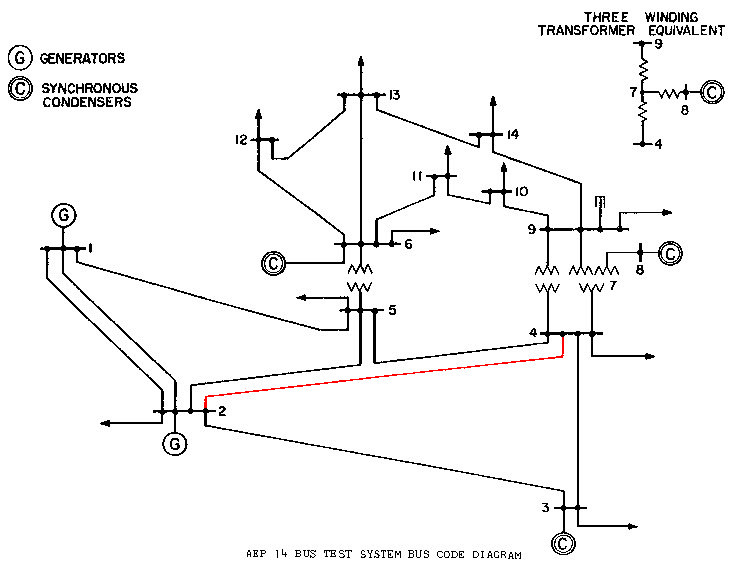
\includegraphics[width=0.60\textwidth]{ieee14.jpg}
  \end{figure}
  We assume $p=1$ and the flow sensor on the red line is being attacked.
\end{frame}


\begin{frame}{Simulation IEEE 14-bus System}
  \begin{figure}[ht]
    \begin{center}
    
      \setlength{\figureheight}{6cm}
      \setlength{\figurewidth}{10cm}
    \definecolor{mycolor1}{rgb}{1.00000,0.00000,1.00000}%
%
\begin{tikzpicture}

\begin{axis}[%
width=\figurewidth,
height=\figureheight,
at={(1.527in,1.083in)},
scale only axis,
xmin=0.95,
xmax=2.4,
xlabel={Normalized MSE of the estimators without attack},
xmajorgrids,
ymin=0.95,
ymax=2.5,
ylabel={Normalized MSE when under attack},
ymajorgrids,
axis background/.style={fill=white},
legend style={at={(0.597,0.528)},anchor=south west,legend cell align=left,align=left,draw=white!15!black}
]
\addplot [color=red,solid,line width=1.5pt,mark=asterisk,mark options={solid}]
  table[row sep=crcr]{%
1.43445926050949	1.60278898169176\\
1.39031186915402	1.55697434518454\\
1.3071172341038	1.45686583321128\\
1.22179873443561	1.39007675912456\\
1.19778876193304	1.39208411785897\\
1.18338657214841	1.41115912951674\\
1.19827557684201	1.43770731227953\\
1.19829876193728	1.45864622150778\\
1.19391115736641	1.47941184470539\\
1.19540182190504	1.49298640841215\\
1.21565436671202	1.5165881854638\\
1.22952576940108	1.54397316883212\\
1.2344017031641	1.57119831765969\\
1.29356861993538	1.63848995702805\\
1.49806241756897	2.01620927014096\\
};
\addlegendentry{$\text{Estimator }\phi$};

\addplot [color=blue,dashed,line width=1.5pt,mark=triangle,mark options={solid}]
  table[row sep=crcr]{%
2.16434829886514	2.41673714136766\\
1.49824142620916	1.6273922047888\\
1.46836558726546	1.61304395019434\\
1.42878218405531	1.58080265845186\\
1.33509034059386	1.48317348510781\\
1.24979953097586	1.4011442907391\\
1.20190884155895	1.36475282176979\\
1.14816845697376	1.32743887772808\\
1.104692902235	1.30458587111275\\
1.0727554366346	1.2930587844785\\
1.04837293442887	1.29286647088633\\
1.03276380632143	1.30464750437787\\
1.02491383863213	1.32636243694814\\
1.0209295289153	1.35606289076979\\
1.01470702949196	1.40680155569416\\
1.00686189169388	1.48274325705327\\
1.00166658882151	1.69020329692052\\
1.00012894457222	2.29806950301701\\
};
\addlegendentry{Estimator g};

\addplot [color=mycolor1,dashed,forget plot]
  table[row sep=crcr]{%
1	1\\
2.2	1\\
};
\addplot [color=mycolor1,dashed,forget plot]
  table[row sep=crcr]{%
1	1\\
1	2.5\\
};
\node[right, align=left, text=blue]
at (axis cs:2.164,2.417) {$\text{   }\leftarrow\text{ }\lambda\rightarrow 0$};
\node[right, align=left, text=blue]
at (axis cs:1.335,1.483) {$\text{   }\leftarrow\text{ }\lambda\text{=0.5}$};
\node[right, align=left, text=blue]
at (axis cs:1.202,1.365) {$\text{   }\leftarrow\text{ }\lambda\text{=1}$};
\node[right, align=left, text=blue]
at (axis cs:1.073,1.293) {$\text{   }\leftarrow\text{ }\lambda\text{=1.9}$};
\node[right, align=left, text=blue]
at (axis cs:1.02,1.356) {$\leftarrow\lambda\text{=3}$};
\node[right, align=left, text=blue]
at (axis cs:1,2.298) {$\text{   }\leftarrow\text{ }\lambda\text{=7}$};
\node[right, align=left, text=red]
at (axis cs:1.434,1.603) {$\text{   }\leftarrow\text{ }\epsilon\text{=0.05}$};
\node[right, align=left, text=red]
at (axis cs:1.03,1.459) {$\epsilon\text{=0.53}\rightarrow\text{   }$};
\node[right, align=left, text=red]
at (axis cs:1.498,2.016) {$\text{   }\leftarrow\text{ }\epsilon\text{=1}$};
\node[right, align=left, text=mycolor1]
at (axis cs:1,2.4) {$\text{   }\leftarrow\text{ LSE}$};
\node[right, align=left, text=mycolor1]
at (axis cs:1.9,1.14) {Oracle LSE};
\node[right, align=left, text=mycolor1]
at (axis cs:1.9,1.07) {$\text{     ~~~~~}\downarrow$};
\end{axis}
\end{tikzpicture}%

    \end{center}
  \end{figure}
\end{frame}
\section{Dynamic State Estimation}
%\frame{\tableofcontents[currentsection]}

\begin{frame}{Dynamic State Estimation}
\begin{enumerate}
\item Consider the following dynamic system
\begin{align}
x(k+1) = A x(k) + w(k),\, y(k) = C x(k) + v(k) + a(k).
\end{align}
\item A linear fixed-gain estimator:
\begin{align}
\hat x(k+1) = A \hat x(k) + K(y(k+1)-CA\hat x(k)),
\end{align}
where $K$ is the estimation gain, and $A-KCA$ is stable.
\begin{center}
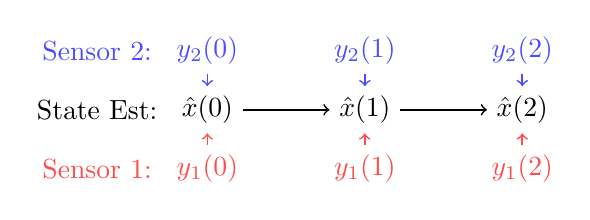
\begin{tikzpicture}[x=2cm, y=0.75cm]
\node at (-0.7,0) {State Est:};
\node [blue!70] at (-0.7,1) {Sensor 2:};
\node [red!70] at (-0.7,-1) {Sensor 1:};

\node            (x0)  at (0,0) {$\hat x(0)$};
\node [blue!70] (y20)  at (0,1)    {$y_2(0)$};
\node [red!70]  (y10)  at (0,-1)   {$y_1(0)$};
\draw [->,semithick,blue!70] (y20) to (x0);
\draw [->,semithick,red!70]  (y10) to (x0);

\node            (x1)  at (1,0) {$\hat x(1)$};
\node [blue!70] (y21)  at (1,1)    {$y_2(1)$};
\node [red!70]  (y11)  at (1,-1)   {$y_1(1)$};
\draw [->,semithick,blue!70] (y21) to (x1);
\draw [->,semithick,red!70]  (y11) to (x1);

\node            (x2)  at (2,0) {$\hat x(2)$};
\node [blue!70] (y22)  at (2,1)    {$y_2(2)$};
\node [red!70]  (y12)  at (2,-1)   {$y_1(2)$};
\draw [->,semithick,blue!70] (y22) to (x2);
\draw [->,semithick,red!70]  (y12) to (x2);

\draw [->,semithick] (x0) to (x1);
\draw [->,semithick] (x1) to (x2);
\end{tikzpicture}
\end{center}
\item The error introduced by the attack may accumulate over time.
\end{enumerate}
\end{frame}

\begin{frame}{Dynamic State Estimate: A Moving Horizon Approach}
In order to convert the dynamic estimation problem into a static one, we can use a moving horizon approach:
\begin{center}
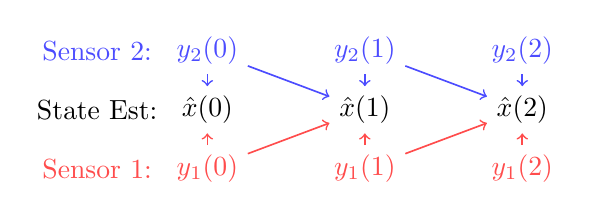
\begin{tikzpicture}[x=2cm, y=0.75cm]
\node at (-0.7,0) {State Est:};
\node [blue!70] at (-0.7,1) {Sensor 2:};
\node [red!70] at (-0.7,-1) {Sensor 1:};

\node            (x0)  at (0,0) {$\hat x(0)$};
\node [blue!70] (y20)  at (0,1)    {$y_2(0)$};
\node [red!70]  (y10)  at (0,-1)   {$y_1(0)$};
\draw [->,semithick,blue!70] (y20) to (x0);
\draw [->,semithick,red!70]  (y10) to (x0);

\node            (x1)  at (1,0) {$\hat x(1)$};
\node [blue!70] (y21)  at (1,1)    {$y_2(1)$};
\node [red!70]  (y11)  at (1,-1)   {$y_1(1)$};
\draw [->,semithick,blue!70] (y21) to (x1);
\draw [->,semithick,red!70]  (y11) to (x1);
\draw [->,semithick,blue!70] (y20) to (x1);
\draw [->,semithick,red!70]  (y10) to (x1);

\node            (x2)  at (2,0) {$\hat x(2)$};
\node [blue!70] (y22)  at (2,1)    {$y_2(2)$};
\node [red!70]  (y12)  at (2,-1)   {$y_1(2)$};
\draw [->,semithick,blue!70] (y22) to (x2);
\draw [->,semithick,red!70]  (y12) to (x2);
\draw [->,semithick,blue!70] (y21) to (x2);
\draw [->,semithick,red!70]  (y11) to (x2);
\end{tikzpicture}
\end{center}

However, the historical data are discarded and the estimation performance may be poor when the system is operating normally.
\end{frame}

\begin{frame}{Dynamic State Estimate: A Local Estimator Approach}
We propose to store historical data in the local estimations:
\begin{center}
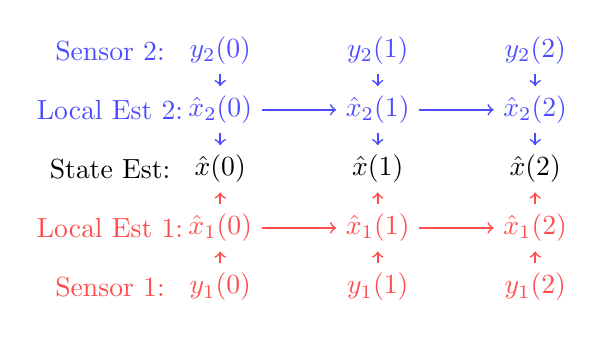
\begin{tikzpicture}[x=2cm, y=0.75cm]
\node at (-0.7,0) {State Est:};
\node [blue!70] at (-0.7,2) {Sensor 2:};
\node [blue!70] at (-0.7,1) {Local Est 2:};
\node [red!70] at (-0.7,-2) {Sensor 1:};
\node [red!70] at (-0.7,-1) {Local Est 1:};

\node            (x0)  at (0,0)    {$\hat x(0)$};
\node [blue!70] (y20)  at (0,2)       {$y_2(0)$};
\node [blue!70] (x20)  at (0,1)  {$\hat x_2(0)$};
\node [red!70]  (y10)  at (0,-2)      {$y_1(0)$};
\node [red!70]  (x10)  at (0,-1) {$\hat x_1(0)$};
\draw [->,semithick,blue!70] (y20) to (x20);
\draw [->,semithick,red!70]  (y10) to (x10);
\draw [->,semithick,blue!70] (x20) to  (x0);
\draw [->,semithick,red!70]  (x10) to  (x0);

\node            (x1)  at (1,0)    {$\hat x(1)$};
\node [blue!70] (y21)  at (1,2)       {$y_2(1)$};
\node [blue!70] (x21)  at (1,1)  {$\hat x_2(1)$};
\node [red!70]  (y11)  at (1,-2)      {$y_1(1)$};
\node [red!70]  (x11)  at (1,-1) {$\hat x_1(1)$};
\draw [->,semithick,blue!70] (y21) to (x21);
\draw [->,semithick,red!70]  (y11) to (x11);
\draw [->,semithick,blue!70] (x21) to  (x1);
\draw [->,semithick,red!70]  (x11) to  (x1);

\node            (x2)  at (2,0)    {$\hat x(2)$};
\node [blue!70] (y22)  at (2,2)       {$y_2(2)$};
\node [blue!70] (x22)  at (2,1)  {$\hat x_2(2)$};
\node [red!70]  (y12)  at (2,-2)      {$y_1(2)$};
\node [red!70]  (x12)  at (2,-1) {$\hat x_1(2)$};
\draw [->,semithick,blue!70] (y22) to (x22);
\draw [->,semithick,red!70]  (y12) to (x12);
\draw [->,semithick,blue!70] (x22) to  (x2);
\draw [->,semithick,red!70]  (x12) to  (x2);

\draw [->,semithick,blue!70] (x20) to (x21);
\draw [->,semithick,blue!70] (x21) to (x22);
\draw [->,semithick,red!70] (x10) to (x11);
\draw [->,semithick,red!70] (x11) to (x12);
\end{tikzpicture}
\end{center}
\begin{enumerate}
\item Construct local estimators (which uses only the local measurements):
\begin{align*}
\hat x_i(k) = A \hat x_i(k) + L_i (y_i(k)-CA\hat x_i(k)).
\end{align*}  
\item Reconstruct the global estimator as
\begin{align*}
\hat x(k) = g(\hat x_1(k),\ldots,\hat x_m(k)).
\end{align*}  
\end{enumerate}
\end{frame}

\begin{frame}{Local Estimator Design}
\begin{enumerate}
\item  Choose $L_i$ such that $A-L_iCA$ shares the same eigenvalues as $A-KCA$.
\begin{align*}
\hat x_i(k) = A \hat x_i(k) + L_i (y_i(k)-CA\hat x_i(k)).
\end{align*}  
\item The global estimate can be recovered as
\begin{align*}
\hat x(k) = F_1\hat x_1(k)+\dots+F_m\hat x_m(k).
\end{align*}
\item More importantly, it can be written as the solution of a quadratic programming problem:
\begin{align*}
  &\mathop{\textrm{minimize}}\limits_{\hat x(k),\hat e(k)}&
  & \frac{1}{2}\hat e(k)^T \tilde W^{-1} \hat e(k)\\
  &\textrm{subject to} &
  &\hat x_i(k)  =  \hat x(k) + \hat e_i(k),&
\end{align*}
\end{enumerate}
\end{frame}

\begin{frame}{Securing the Global Estimate}
We can secure the global estimator using LASSO:
\begin{align*}
  &\mathop{\textrm{minimize}}\limits_{\hat x(k),\hat e(k)}&
  & \frac{1}{2}\hat e(k)^T \tilde W^{-1} \hat e(k) + \gamma \sum_{i=1}^m \|\hat \nu_i(k)\|_1\\
  &\textrm{subject to} &
  &\hat x_i(k)  =  \hat x(k) + \hat e_i(k)+\hat \nu_i(k),&
\end{align*}
One can prove the following:
\begin{enumerate}
\item If there is no attack, then the LASSO will recover the original estimate if the local estimation error belongs to a polytope (scaled with $\gamma$).
\item If there is an attack and less than one half of the sensors are malicious, then the estimator is still stable.
\end{enumerate}
\end{frame}
\section{Conclusion}
\begin{frame}{Conclusion}
% We consider two different information fusion schemes: state estimation and average consensus and design low weight algorithms to address the security and privacy challenges in these settings.
  We consider the problem of state estimation in the presence of malicious sensors and design algorithms to detect and identify the set of compromised sensors and generate stable state estimate against all possible attacks.
\end{frame}

\begin{frame}[standout]
  Thank you!
\end{frame}



\end{document}
